\documentclass{article}
\usepackage[T1]{fontenc}
\usepackage{lmodern}
\usepackage{graphicx}
\usepackage{amsmath,amssymb}
\usepackage[a4paper,margin=2cm]{geometry}
\usepackage[absolute,overlay]{textpos}
\setlength{\TPHorizModule}{1mm}
\setlength{\TPVertModule}{1mm}
\usepackage[indonesian]{babel}
\usepackage{hyperref}
\setlength{\emergencystretch}{2em}
% unit: Halaman 48

\begin{document}

% === Halaman 48 (python/native) ===

48

Contoh 1:

• Tinjau 1 buah pixel dari citra 24-bit (3 x 8 bit):



10000010 

  01111011 

01110101


                   (130)                         (123) 

     (117) 

• Bit bit-bit embedded message:  101  

• Embed:      00110011 

10100010 

11100011 


Original: misalkan pixel  [130, 123, 117] berwarna “ungu”

Stego-image: pixel  [131, 122, 117] tetap “ungu” tapi berubah sangat sedikit. 

Mata manusia tidak dapat membedakan perubahan warna yang sangat kecil. 

Stego-image

% deskripsi: gambar native xref 225
\noindent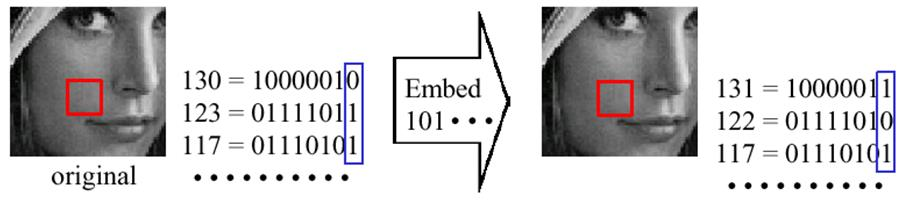
\includegraphics[width=0.85\textwidth]{../../images/python/page_048_img_01.jpeg}

\end{document}
